\newpage
\section{Trigonometry}

\hfill \break
\subsection{Strahlensatz}

\hfill \break
Werden zwei von einem Punkt ausgehende Strahlen von zwei Parallellen Geschnitten, so lassen sich daraus bestimmte Verhältnisse abslesen. $\rightarrow$ Strahlensätze


\hfill \break
Regeln:
\begin{itemize}
    \item $a:b=c:d$
    \item $b*c=a*d$
\end{itemize}


\hfill \break
Beispiel für Strahlensätze:

\hfill \break
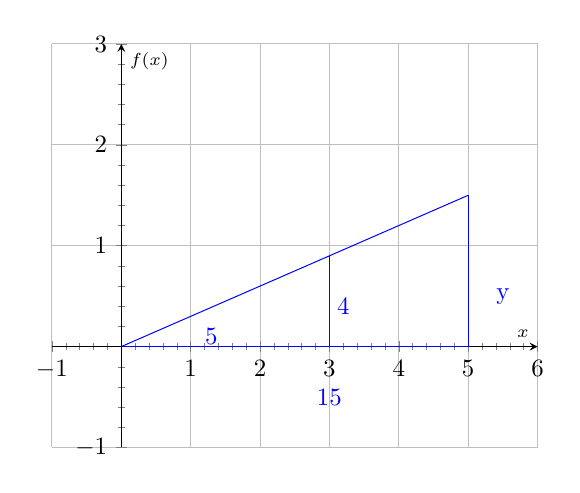
\begin{tikzpicture}[scale=0.9]
    \begin{axis}%
        [
            grid=major,
            xtick={-1,0,...,7},
            minor x tick num=4, % 4 minor ticks => 5 subintervals
            xmin=-1,
            xmax=6,
            xlabel={\scriptsize $x$},
            axis x line=middle,
            ytick={-1,0,...,3},
            minor y tick num=4,  % 4 minor ticks => 5 subintervals
            ymin=-1,
            ymax=3,
            ylabel={\scriptsize $f(x)$},
            axis y line=middle,
            no markers,
            samples=100,
            domain=-6:6,
        ]

        \draw[color=blue] (0,0) -- (5,1.5);
        \draw[color=blue] (5,0) -- (5,1.5);
        \draw[color=blue] (5,0) -- (0,0);
        \draw[color=blue] (3,0) -- (3,0.9);
        \node[color=blue] at (1.3,0.1) {5};
        \node[color=blue] at (3,-0.5) {15};
        \node[color=blue] at (5.5,0.5) {y};
        \node[color=blue] at (3.2,0.4) {4};
    \end{axis}
\end{tikzpicture}

\hfill \break
Example Verhältnisgleichung:\\
\fboxrule=0.8pt \fcolorbox{black}{lightgray}{%
    \begin{tabular}[t]{@{}l@{}}
        $5:4 = 15:y$ \\
        $5y = 60$    \\
        $y = 12$     \\
    \end{tabular}}

\break
\newpage
\subsection{Decimal und Sexagesimalsystem}

\hfill \break
\fboxrule=0.8pt \fcolorbox{lightgray}{lightgray}{%
    \begin{tabular}{c||c}
        \textcolor{red}{Decimal (Basis 10)} & \textcolor{blue}{Sexagesimal (Basis 60)} \\
        \hline
        $6.5$ h                             & 6h 30min                                 \\
        $20.1$ h                            & 20h 6min                                \\
        $19.815$ h                          & 19h 48min                                \\
    \end{tabular}}\\


\hfill \break
Umrechnung von Grad zu Rad
\begin{itemize}
    \item Grad einegben zb: $19.815$
    \item $2nd$ Angle
    \item Punkt 4 $\rightarrow$ DMS
\end{itemize}

\hfill \break
Umrechnung von Rad zu Grad
\begin{itemize}
    \item Rad einegben zb: $19^{\circ}48'54"$ die einheiten $^{\circ}$ ' können unter $2nd$ Angl gefunden werden
    \item das Zeichen " gibt es unter Alpha +
\end{itemize}

\break
\input{Topics/Trigonometry/SubTopics/Bogenmaß}
\break
\newpage
\subsection{Sinus, Cosinus und Tangens}

\hfill \break
Der Einheitskreis ist ein Kreis mir einem Radius von der Länge 1. Es wird keine Einheit angegeben.

\hfill \break
\begin{itemize}
    \item $Sin(\alpha) = \frac{\textcolor{red}{3}}{\textcolor{purple}{5}} = \frac{\textcolor{cyan}{6}}{\textcolor{violet}{7.5}}= \frac{\textcolor{cyan}{Gegenkatete}}{\textcolor{violet}{Hypothenuse}}$
    \item $Cos(\alpha) = \frac{\textcolor{green}{4}}{\textcolor{purple}{5}} = \frac{\textcolor{olive}{8}}{\textcolor{violet}{7.5}}= \frac{\textcolor{olive}{Ankatete}}{\textcolor{violet}{Hypothenuse}}$
    \item $Tan(\alpha) = \frac{\textcolor{red}{3}}{\textcolor{green}{4}} = \frac{\textcolor{cyan}{6}}{\textcolor{olive}{8}} = \frac{\textcolor{cyan}{Gegenkatete}}{\textcolor{olive}{Ankatete}}$
\end{itemize}


\hfill \break
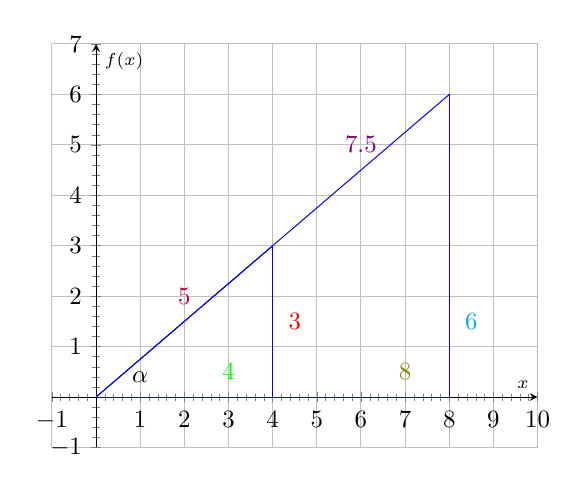
\begin{tikzpicture}[scale=0.9]
    \begin{axis}%
        [
            grid=major,
            xtick={-1,0,...,10},
            minor x tick num=4, % 4 minor ticks => 5 subintervals
            xmin=-1,
            xmax=10,
            xlabel={\scriptsize $x$},
            axis x line=middle,
            ytick={-1,0,...,7},
            minor y tick num=4,  % 4 minor ticks => 5 subintervals
            ymin=-1,
            ymax=7,
            ylabel={\scriptsize $f(x)$},
            axis y line=middle,
            no markers,
            samples=100,
            domain=-6:6,
        ]

        \draw[color=blue] (0,0) -- (8,6);
        \draw[color=blue] (0,0) -- (4,3);
        \draw[color=blue] (8,0) -- (8,6);
        \draw[color=blue] (4,0) -- (4,3);
        \draw[color=blue] (4,0) -- (0,0);
        \draw[color=blue] (8,0) -- (0,0);

        \node[color=black] at (1,0.4) {$\alpha$};

        \node[color=purple] at (2,2) {$5$};
        \node[color=violet] at (6,5) {$7.5$};
        \node[color=red] at (4.5,1.5) {$3$};
        \node[color=cyan] at (8.5,1.5) {$6$};
        \node[color=green] at (3,0.5) {$4$};
        \node[color=olive] at (7,0.5) {$8$};
    \end{axis}
\end{tikzpicture}


\hfill \break
Die Umkehrung vom Sinus ist der Arkussinus.


\hfill \break
Example zum errechnen von $\alpha$:\\
\fboxrule=0.8pt \fcolorbox{black}{lightgray}{%
    \begin{tabular}[t]{@{}l@{}}
        $Sin(\alpha) = 0.6$ // Te $\rightarrow$ $sin^{-1}$ \\
        $\alpha = 36.87^{\circ}$                           \\
        \\
        \\
        $Cos(\alpha) = 0.8$ // Te $\rightarrow$ $cos^{-1}$ \\
        $\alpha = 36.87^{\circ}$
    \end{tabular}}

\break
\newpage
\subsection{Die Winkelfunktionen}

\hfill \break
\begin{itemize}
    \item $Sin(\alpha) = \frac{GK}{H} = \frac{GK}{1} = GK$
    \item $Cos(\alpha) = \frac{AK}{H} = \frac{AK}{1} = AK$
    \item 
    \item $Tan(\alpha) = \frac{GK}{AK} = \frac{\frac{sin(\alpha)}{cos(\alpha)}}{AK}$
\end{itemize}

\hfill \break
\begin{enumerate}
    \item Trigonometriesche Grundbeziehung = $\frac{tan(\alpha)}{1} = \frac{sin(\alpha)}{cos(\alpha)}$
    \item Pythagoras = $1 = sin(\alpha)^2 + cos(\alpha)^2$
\end{enumerate}



\hfill \break
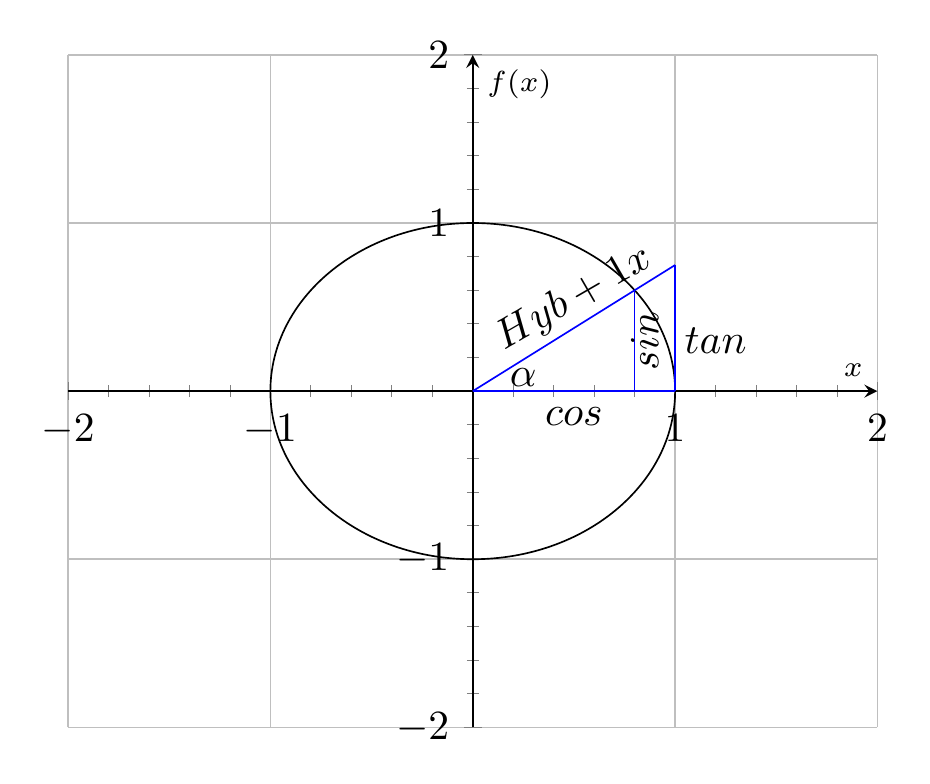
\begin{tikzpicture}[scale=1.5]
    \begin{axis}%
        [
            grid=major,
            xtick={-2,-1,...,2},
            minor x tick num=4,
            xmin=-2,
            xmax=2,
            xlabel={\scriptsize $x$},
            axis x line=middle,
            ytick={-2,-1,...,2},
            minor y tick num=4, 
            ymin=-2,
            ymax=2,
            ylabel={\scriptsize $f(x)$},
            axis y line=middle,
            no markers,
            samples=100,
            domain=-6:6,
        ]

        \draw[] (0,0) circle (1);
        \draw[color=blue] (0,0) -- (0.8,0.6);
        \draw[color=blue] (0.8,0) -- (0.8,0.6);
        \draw[color=blue] (0,0) -- (0.8,0);
        \draw[color=blue] (0.8,0.6) -- (1,0.75);
        \draw[color=blue] (1,0) -- (1,0.75);
        \draw[color=blue] (0.8,0) -- (1,0);


        \node[] at (0.25,0.08) {$\alpha$};
        \node[] at (0.5,-0.15) {$cos$};
        \node[rotate=90] at (0.85,0.3) {$sin$};
        \node[] at (1.2,0.3) {$tan$};
        \node[rotate=30] at (0.5,0.55) {$Hyb + 1x$};

    \end{axis}
\end{tikzpicture}
\break
\newpage
\subsection{Schwingungen}

\hfill \break
Die Werte von Sin und Cos können nie kleiner als -1 und größers als 1 werden.\\
Überträgt man die Längen (AK/GK) mit den dazu gehörigen Winkeln in ein Koordinatensystem, erhällt man folgende Funktionsgraphen:


\hfill \break
\subsubsection{Die Sinus Funktion}

\begin{itemize}
    \item $sin(deg(x))$
    \item diese Funktion hat eine Periode von $2*\pi$
\end{itemize}


\hfill \break
Die Wertetabelle und Graphik zu $sin(deg(x))$:\\
\fboxrule=0.8pt \fcolorbox{lightgray}{lightgray}{%
    \begin{tabular}{c|c}
        $x$               & $y$ \\
        \hline
        $0$               & 0   \\
        $\frac{\pi}{2}$   & 1   \\
        $\pi$             & 0   \\
        $\frac{3*\pi}{2}$ & -1  \\
        $2*\pi$           & 0   \\
    \end{tabular}}\\


\hfill \break
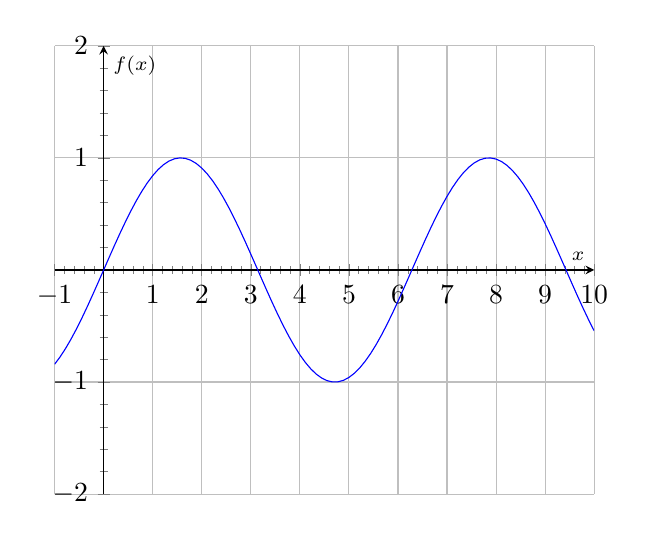
\begin{tikzpicture}[scale=1]
    \begin{axis}%
        [
            grid=major,
            xtick={-1,0,...,10},
            minor x tick num=4,
            xmin=-1,
            xmax=10,
            xlabel={\scriptsize $x$},
            axis x line=middle,
            ytick={-2,-4,...,2},
            minor y tick num=4,
            ymin=-2,
            ymax=2,
            ylabel={\scriptsize $f(x)$},
            axis y line=middle,
            no markers,
            samples=100,
            domain=-1:10,
        ]
        \addplot[blue] (x,{sin(deg(x))});
    \end{axis}
\end{tikzpicture}
\break
\newpage
\subsubsection{Die Kosinus Funktion}

\begin{itemize}
    \item $cos(deg(x))$
    \item diese Funktion hat eine Periode von $2*\pi$
\end{itemize}


\hfill \break
Die Wertetabelle und Graphik zu $cos(deg(x))$:\\
\fboxrule=0.8pt \fcolorbox{lightgray}{lightgray}{%
    \begin{tabular}{c|c}
        $x$               & $y$ \\
        \hline
        $0$               & 1   \\
        $\frac{\pi}{2}$   & 0   \\
        $\pi$             & -1   \\
        $\frac{3*\pi}{2}$ & 0  \\
        $2*\pi$           & 1   \\
    \end{tabular}}\\


\hfill \break
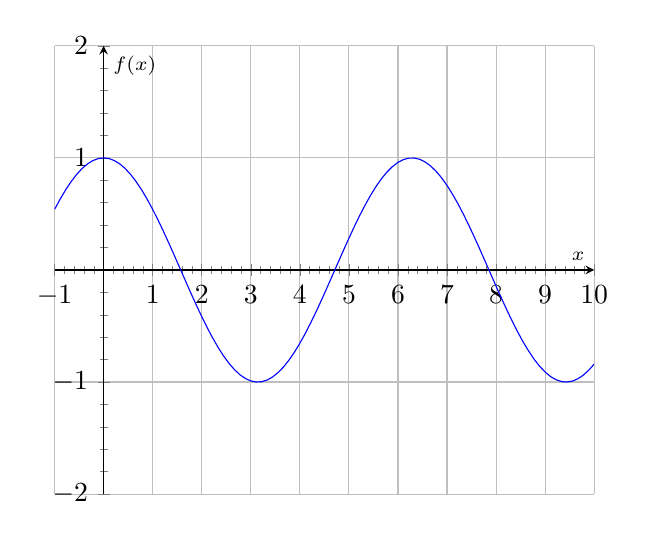
\begin{tikzpicture}[scale=1]
    \begin{axis}%
        [
            grid=major,
            xtick={-1,0,...,10},
            minor x tick num=4,
            xmin=-1,
            xmax=10,
            xlabel={\scriptsize $x$},
            axis x line=middle,
            ytick={-2,-4,...,2},
            minor y tick num=4,
            ymin=-2,
            ymax=2,
            ylabel={\scriptsize $f(x)$},
            axis y line=middle,
            no markers,
            samples=100,
            domain=-1:10,
        ]
        \addplot[blue] (x,{cos(deg(x))});
    \end{axis}
\end{tikzpicture}
\break
\newpage
\subsubsection{Die Tangens Funktion}

\begin{itemize}
    \item $tan(deg(x))$
    \item Tangens ist ein Sonderfall bezüglich des Vorzeichens.
\end{itemize}


\hfill \break
Die Wertetabelle und Graphik zu $tan(deg(x))$:\\
\fboxrule=0.8pt \fcolorbox{lightgray}{lightgray}{%
    \begin{tabular}{c|c}
        $x$               & $y$ \\
        \hline
        $0$               & 0   \\
        $\frac{\pi}{2}$   & n.d.   \\
        $\pi$             & 0   \\
        $\frac{3*\pi}{2}$ & n.d.   \\
        $2*\pi$           & 0   \\
    \end{tabular}}\\


\hfill \break
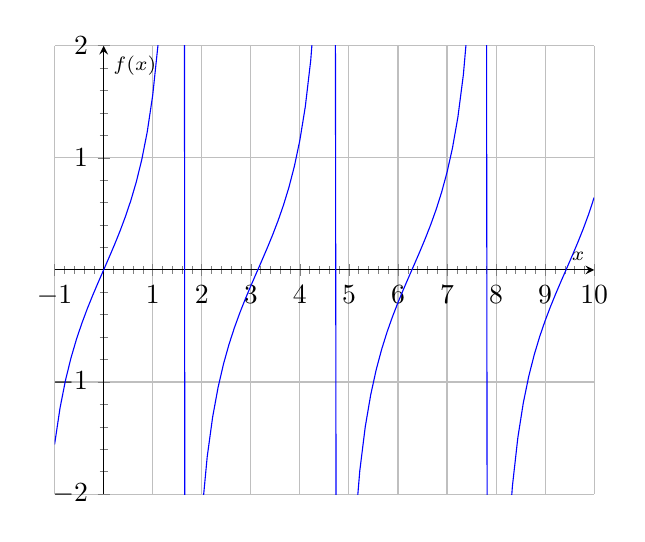
\begin{tikzpicture}[scale=1]
    \begin{axis}%
        [
            grid=major,
            xtick={-1,0,...,10},
            minor x tick num=4,
            xmin=-1,
            xmax=10,
            xlabel={\scriptsize $x$},
            axis x line=middle,
            ytick={-2,-4,...,2},
            minor y tick num=4,
            ymin=-2,
            ymax=2,
            ylabel={\scriptsize $f(x)$},
            axis y line=middle,
            no markers,
            samples=100,
            domain=-1:10,
        ]
        \addplot[blue] (x,{tan(deg(x))});
    \end{axis}
\end{tikzpicture}
\break
\input{Topics/Trigonometry/SubTopics/VeränderungDerSinFunktion}
\break
\newpage
\subsection{Sinus und Kosinussatz und Fläche}

\hfill \break
In jedem Dreieck verhalten sich die Längen zweier Seiten wie die Sienuswerte der gegenüberliegenden Winkel.

\hfill \break
\begin{itemize}
    \item 1.Sinussatz $\rightarrow \frac{sin(\alpha)}{a}$
    \item 2.Sinussatz $\rightarrow \frac{sin(\beta)}{b}$
    \item 3.Sinussatz $\rightarrow \frac{sin(\gamma)}{c}$
    \item 1.Kosinussatz $\rightarrow c^2 = a^2 + b^2 +2*a*b*cos(\gamma)$
    \item 2.Kosinussatz $\rightarrow b^2 = a^2 + c^2 +2*a*c*cos(\beta)$
    \item 3.Kosinussatz $\rightarrow a^2 = b^2 + c^2 +2*b*c*cos(\alpha)$
    \item Fläche im algemeinen Dreieck $\rightarrow A = \frac{a*ha}{2}$
    \item Fläche im algemeinen Dreieck $\rightarrow A = \frac{c*b*sin(\alpha)}{2}$
\end{itemize}

\break
\newpage
\subsection{Allgemeines Dreieck}

\begin{itemize}
    \item $sin(\alpha) = \frac{hc}{b} \rightarrow hc = sin(\alpha)*b \rightarrow hc$
    \item $sin(\beta) = \frac{hc}{a} \rightarrow hc = sin(\beta)*a \rightarrow hc$
    \item $sin(\alpha)*b = sin(\beta)*a$
    \item $\frac{sin(\alpha)}{a} = \frac{sin(\beta)}{b}$
    \item $A=\frac{b*c}{2} * sin(\alpha)$
    \item $A=\frac{a*c}{2} * sin(\beta)$
    \item $A=\frac{a*b}{2} * sin(\gamma)$
\end{itemize}

\hfill \break
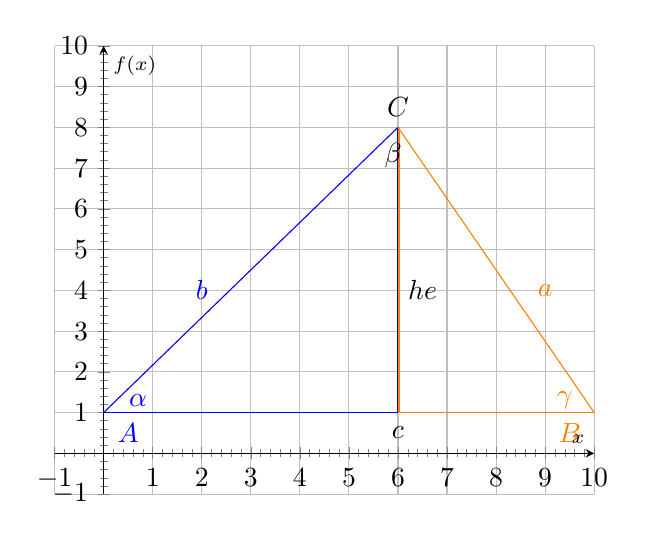
\begin{tikzpicture}[scale=1]
    \begin{axis}%
        [
            grid=major,
            xtick={-1,0,...,10},
            minor x tick num=4,
            xmin=-1,
            xmax=10,
            xlabel={\scriptsize $x$},
            axis x line=middle,
            ytick={-1,0,...,10},
            minor y tick num=4,
            ymin=-1,
            ymax=10,
            ylabel={\scriptsize $f(x)$},
            axis y line=middle,
            no markers,
            samples=100,
            domain=-1:10,
        ]

        \draw[color=blue] (0,1) -- (6,8);
        \draw[color=blue] (0,1) -- (6,1);
        \draw[color=blue] (5.99,1) -- (5.99,8);
        \draw[color=orange] (6.02,1) -- (6.02,8);
        \draw[color=orange] (10,1) -- (6,8);
        \draw[color=orange] (6,1) -- (10,1);

        \node[color=blue] at (0.7,1.3) {$\alpha$};
        \node[color=black] at (5.9,7.3) {$\beta$};
        \node[color=orange] at (9.4,1.3) {$\gamma$};

        \node[color=black] at (6.5,4) {$he$};
        \node[color=orange] at (9,4) {$a$};
        \node[color=blue] at (2,4) {$b$};
        \node[color=black] at (6,0.5) {$c$};

        \node[color=blue] at (0.5,0.5) {$A$};
        \node[color=orange] at (9.5,0.5) {$B$};
        \node[color=black] at (6,8.5) {$C$};
    \end{axis}
\end{tikzpicture}
\break
\newpage
\subsection{Vermessungsaufgaben}


\hfill \break
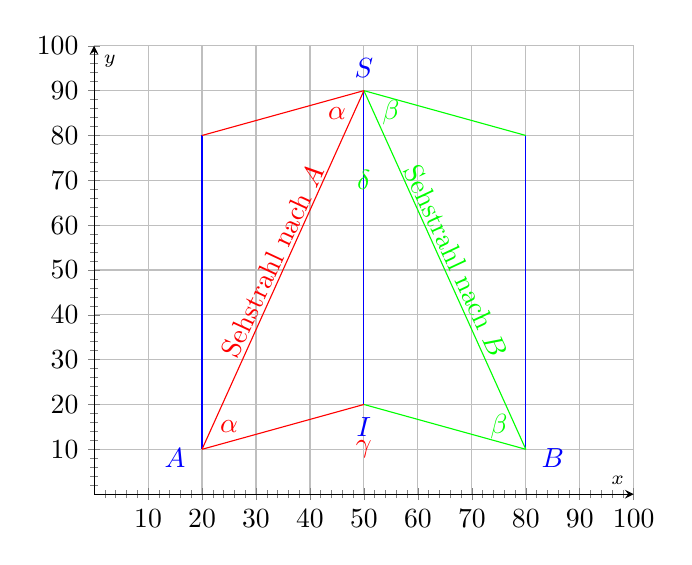
\begin{tikzpicture}[scale=1]
    \begin{axis}%
        [
            grid=major,
            xtick={0,10,...,100},
            minor x tick num=4,
            xmin=0,
            xmax=100,
            xlabel={\scriptsize $x$},
            axis x line=middle,
            ytick={0,10,...,100},
            minor y tick num=4,
            ymin=0,
            ymax=100,
            ylabel={\scriptsize $y$},
            axis y line=middle,
            no markers,
            samples=100,
            domain=-1:10,
        ]

        \draw[color=blue] (50,20) -- (50,90);
        \draw[color=blue] (20,10) -- (20,80);
        \draw[color=blue] (80,10) -- (80,80);
        \draw[color=green] (80,80) -- (50,90);
        \draw[color=green] (80,10) -- (50,20);
        \draw[color=green] (80,10) -- (50,90);
        \draw[color=red] (20,80) -- (50,90);
        \draw[color=red] (20,10) -- (50,20);
        \draw[color=red] (20,10) -- (50,90);

        \node[color=green,rotate=-65] at (67,52) {Sehstrahl nach $B$};
        \node[color=red,rotate=65] at (33,52) {Sehstrahl nach $A$};

        \node[color=red] at (25,15) {$\alpha$};
        \node[color=green] at (75,15) {$\beta$};
        \node[color=red] at (45,85) {$\alpha$};
        \node[color=green] at (55,85) {$\beta$};

        \node[color=red] at (50,10) {$\gamma$};
        \node[color=green] at (50,70) {$\delta$};
        \node[color=blue] at (15,8) {$A$};
        \node[color=blue] at (85,8) {$B$};
        \node[color=blue] at (50,95) {$S$};
        \node[color=blue] at (50,15) {$I$};


    \end{axis}
\end{tikzpicture}


\hfill \break
\begin{itemize}
    \item $\textcolor{red}{\alpha},\textcolor{green}{\beta} \rightarrow$ Hähenwinkel, von der Horizontale aus nach oben gemessen.
    \item $\textcolor{red}{\alpha},\textcolor{green}{\beta} \rightarrow$ Tiefenwinkel, von der Horizontale aus nach unten gemessen.
    \item $\textcolor{red}{\gamma}... Horizontalwinkel$ zwischen den 2 gedachten Linien.
    \item $\textcolor{green}{\delta}... Sehwinkel$ von 2 Sehstralen.
\end{itemize}

\newpage
\subsubsection{Beispiel 1: Der Fluss}

\hfill \break
Berechne die Breite eines Flusses, wenn in einem geradlinigen Uferstück die Standlinie AB (150m) abgesteckt wird
sowie die Winkel CAB (63°22') und CBA (44°30') zu einem am gegenüberliegenden Ufer liegenden Punkt C gemessen
wird.
(Lösung: 98,75m)

\hfill \break
\begin{itemize}
    \item Winkel $CAB = \alpha = 63.37$°
    \item Winkel $CBA = \beta = 44.5$°
    \item Winkel $BC = \gamma = 72.13$°
\end{itemize}

\hfill \break
Rechenweg:\\
\fboxrule=0.8pt \fcolorbox{black}{lightgray}{%
    \begin{tabular}[t]{@{}l@{}}
        $x = \frac{Sin(44.5)*150}{Sin(72.13)}$ \\
        $x = 110.47$                           \\
        \\
        $b=Sin(\alpha)/x$                      \\
        $b=Sin(63.37)*110.47$                  \\
        $b=98.75m$                              \\
    \end{tabular}}

\hfill \break
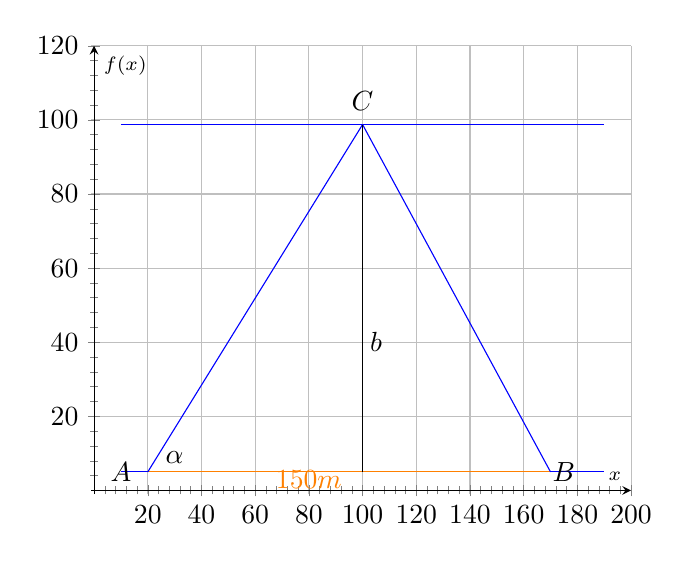
\begin{tikzpicture}[scale=1]
    \begin{axis}%
        [
            grid=major,
            xtick={0,20,...,200},
            minor x tick num=4,
            xmin=-1,
            xmax=200,
            xlabel={\scriptsize $x$},
            axis x line=middle,
            ytick={0,20,...,120},
            minor y tick num=4,
            ymin=-1,
            ymax=120,
            ylabel={\scriptsize $f(x)$},
            axis y line=middle,
            no markers,
            samples=100,
            domain=-1:10,
        ]

        \draw[color=blue] (10,5) -- (190,5);
        \draw[color=orange] (20,5) -- (170,5);
        \draw[color=blue] (10,98.75) -- (190,98.75);
        \draw[color=blue] (100,98.75) -- (20,5);
        \draw[color=blue] (100,98.75) -- (170,5);
        \draw[color=black] (100,98.75) -- (100,5);

        \node[color=black] at (10,5) {$A$};
        \node[color=black] at (175,5) {$B$};
        \node[color=black] at (100,105) {$C$};
        \node[color=black] at (105,40) {$b$};
        \node[color=black] at (30,9) {$\alpha$};
        \node[color=orange] at (80,3) {$150m$};
    \end{axis}
\end{tikzpicture}
\newpage
\subsubsection{Beispiel 2: Der Antennemast}

\hfill \break
Der Antennenmast eines Fernsehturms hat die Höhe h = 75m. Von einem Geländepunkt P werden Spitze und Fußpunkt
des Antennenmast unter den Höhenwinkeln a = 24°12' und ß = 17°42' gesehen. Ermittle die Höhe des Fernsehturms
mit Sendemast.
(Lösung: 258,73m)

\hfill \break
\begin{itemize}
    \item Winkel $\alpha = 24.2$°
    \item Winkel $\beta = 17+\frac{42}{60}$°
    \item Winkel $\gamma = 24.2-1.7=6.5$°
    \item Winkel $\delta = 180 - 90 - 17.7 = 72.3$°
    \item Winkel $\epsilon = 107.7$°
    \item Winkel $\zeta = 65.8$°
\end{itemize}

\hfill \break
Rechenweg:\\
\fboxrule=0.8pt \fcolorbox{black}{lightgray}{%
    \begin{tabular}[t]{@{}l@{}}
        $\frac{75}{Sin(\alpha)} = \frac{\gamma}{Sin(\zeta)}$ \\
        $\frac{75}{Sin(\alpha)} = \gamma$                    \\
        $y = 604.3$                                          \\
        \\
        $Sin(\beta) = \frac{x}{y}$                           \\
        $Sin(\beta)*\gamma = x$                              \\
        $x = 183.73$                                         \\
        \\
        $H = 183.73 + 75 = 258.73$                           \\
    \end{tabular}}

%//TODO add drawing